\documentclass[openany,12pt]{memoir}
\usepackage{amsmath}
\usepackage{amssymb}
\usepackage{amsthm}
\usepackage{authblk}
\usepackage{xcolor}
\usepackage[framemethod=tikz]{mdframed}
\usepackage{tikz}
\usepackage{enumitem}
\usepackage{fancyhdr}
\usepackage{calc}
\usepackage{marginnote}
\usepackage{graphicx}
\usepackage{hyperref}


% Setting Biblatex Styles
\bibliographystyle{plain}
\nocite{*} % Include all entries from the BibTeX file
\let\cleardoublepage\clearpage
\renewcommand{\bibname}{\Large{References}}
\renewcommand{\bibsection}{%
  \section*{\bibname}% Use \section* to suppress numbering
  \markboth{\MakeUppercase{\bibname}}{\MakeUppercase{\bibname}}%
}

%%%%%%%%%%%%%%%%%%%%%%%%%%%%%%%%%%%%%%%%%%%%%%%%%%%%%%%%%%%%%%%%%%%%%%%%%%%%%%%%%%%
%                       DEFINING THE THEOREM ENVIRONMENT                          %
% The Theorem environment 'thm' has a vertical black line to the left of the box  %
%                                                                                 %
\newtheorem*{thm}{Theorem}                                                         %
\surroundwithmdframed[outerlinecolor=white,outerlinewidth=2pt,innerlinewidth=4pt, %
  bottomline=false,topline=false,rightline=false]{thm}                            %
%%%%%%%%%%%%%%%%%%%%%%%%%%%%%%%%%%%%%%%%%%%%%%%%%%%%%%%%%%%%%%%%%%%%%%%%%%%%%%%%%%%

% Set the left and right margin for the header
\pagestyle{fancy}
\fancyhf{} % Empty Headers
\fancyhead[LE]{\thepage} % Page number on left for even pages
\fancyhead[RO]{\thepage} % Page number on right for odd pages
\fancyhead[RE]{\textit{Communicating without errors}} % Header on even pages
\fancyhead[LO]{\textit{Communicating without errors}} % Header on odd pages

% REMOVE ALL INDENTATION ON PARAGRAPHS
\setlength{\parindent}{0pt}

% REDEFINE \theequation TO EXCLUDE CHAPTER NUMBER
\renewcommand{\theequation}{\arabic{equation}}

% DEFINE ENVIRONMENT FOR QUOTES
\newmdenv[
  backgroundcolor=white,
  linewidth=0pt,
  innerleftmargin=8pt,
  innertopmargin=10pt,
  innerrightmargin=0pt,
  innerbottommargin=10pt,
  leftmargin=-10pt,
  skipabove=\topsep,
  skipbelow=\topsep,
  frametitle={\tikz[overlay,remember picture] \node[anchor=north east,rectangle,fill=gray!60,inner sep=4pt] at (frame.north east) {};}
]{quotebox}

\newenvironment{myquote}
{\begin{quotebox}\begin{quote}}
{\end{quote}\end{quotebox}}

% DEFINE DOCUMENT MARGINS
\setlrmarginsandblock{0.5cm}{8cm}{*}
\setulmarginsandblock{0}{0cm}{*}
\checkandfixthelayout

% DEFINE MARGINS FOR NEW PAGES
\newcommand{\setnewpagemargins}{
    \clearpage
    \setulmarginsandblock{2cm}{0.5cm}{*}
    \checkandfixthelayout
}

% SET UP BOX LINE WIDTH
\mdfsetup{linewidth=1pt}

%% SET CORRECT CHAPTER AND PAGE NUMBERS %%
\setcounter{chapter}{32}
\setcounter{page}{213} % FIX PAGE NUMBERING %

% ADJUST SPACE BEFORE AND AFTER CHAPTER TITLE
\setlength{\beforechapskip}{5pt}
\setlength{\afterchapskip}{55pt}

% BEGINNING DOCUMENT
\begin{document}

\chapter{Communicating without errors}

% Add TWO IMAGES IN THE RIGHT MARGIN
\marginnote{\hspace*{10pt}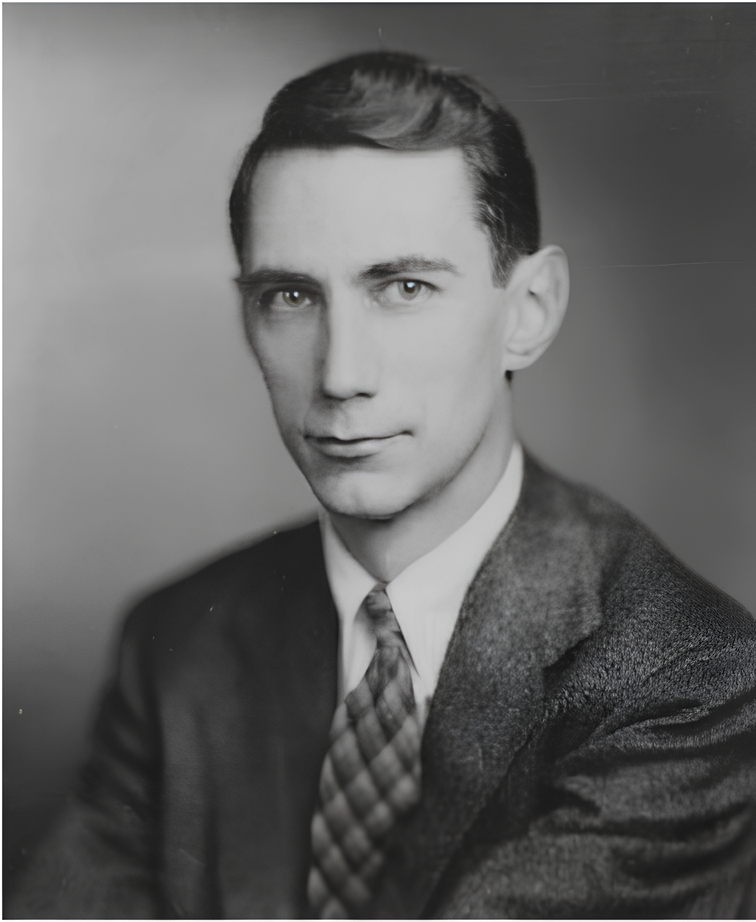
\includegraphics[width=\marginparwidth-30pt]{images/shannon.jpg}\\\hspace*{10pt}Claude Shannon}[0pt]
\marginnote{\hspace*{0pt}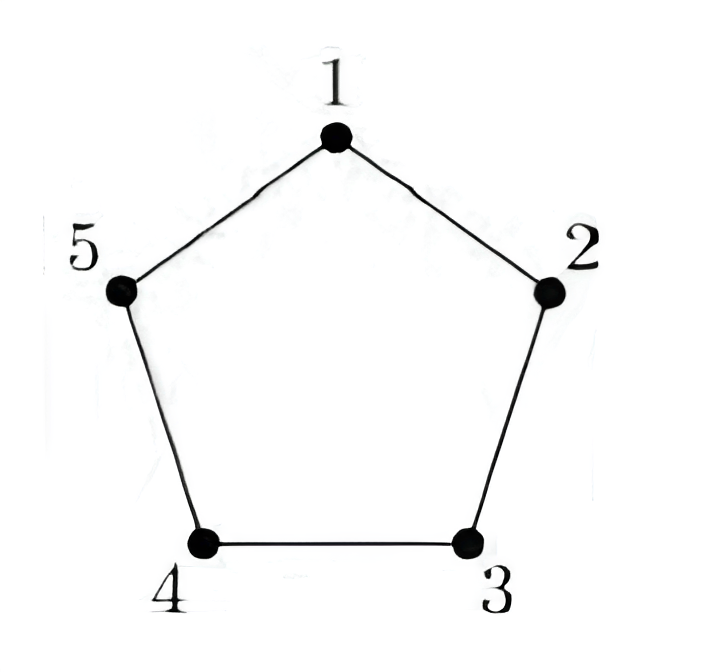
\includegraphics[width=125pt]{images/C5.png}}[267pt]

In 1956 Claude Shannon, the founder of information theory, posed the following very interesting question:

\begin{myquote}
\textit{Suppose we want to transmit messages across a channel (where
some symbols may be distorted) to a receiver: What is the maximum
rate of transmission such that the receiver may recover the original
message without errors?}
\end{myquote}

Let us see what Shannon meant by ``channel" and ``rate of transmission." 
We are given a set V of symbols, and a message is just a string of symbols 
from V. We model the channel as a graph $G = (V,E)$  where $V$ is the set 
of symbols, and $E$ the set of edges between unreliable pairs of symbols, 
that is, symbols which may be confused during transmission. For example, 
communicating over a phone in everyday language, we connnect the symbols
$B$ and $P$ by an edge since the receiver may not be able to distinguish 
them. Let us call $G$ the \textit{confusion graph}.
The 5-cycle $C_5$ will play a prominent role in our discussion. In this example,
$1$ and $2$ may be confused, but not $1$ and $3$, etc. Ideally we would like 
to use all $5$ symbols for transmission, but since we want to communicate error-free we can 
if we only send single symbols use only one letter from each pair that might
be confused. Thus for the 5-cycle we can use only two different letters
(any two that are not connected by an edge). In the language of information theory,
this means that for the 5-cycle we achieve an information rate of
$\log_2 2 = 1$ (instead of the maximal $\log_2 5 \approx 2.32$). It is clear that in this model,
for an arbitrary graph $G = (V, E)$, the best we can do is to transmit symbols from
a largest independent set. Thus the information rate, when sending single symbols,
is $log_2 \alpha(G)$, where $\alpha(G)$ is the \textit{independence number} of $G$.

Let us see whether we can increase the information rate by using larger 
strings in place of single symbols. Suppose we want to transmit strings of 
length 2. The strings ulu2 and vlv, can only be confused if one of the 
following three cases holds: 

\begin{itemize}[leftmargin=12pt]
  \item $u_1 = v_1$ and $u_2$ can be confused with $v_2$,
  \item $u_2 = v_2$ and $u_1$ can be confused with $v_1$, or
  \item $u_1 \neq v_1$ can be confused and $u_2 \neq v_2$ can be confused. 
\end{itemize}

In graph-theoretic terms this amounts to considering the product $G_1 \times G_2$ 
of two graphs $G_1 = (V_1, E_1)$  and $G_2 = (V_1, E_1)$. $G_1 \times G_2$ has the vertex

%%%%%%%%%%%%%%%%%%%%%%%%%%%%%%%%%%%%%%%%%%%%%%%%%%
% SECOND PAGE
\setnewpagemargins

set $V_1 \times V_2 = \{(u_1,u_2) :\ u_1 \in V_1,u_2 \in V_2\}$, with $(u_1,u_2) \neq (v_1,v_2)$ 
connected by an edge if and only if $u_i = v_i$ or $u_iv_i \in E$ for $i = 1,2$. The 
confusion graph for strings of length $2$ is thus $G^2 - G \times G$, the product of 
the confusion graph $G$ for single symbols with itself. The information rate 
of strings of length $2$ \textit{per symbol} is then given by

\begin{equation*}
  \frac{\log_2 \alpha(G^2)}{2} = \log_2\sqrt{\alpha(G^2)}.
\end{equation*}

Now, of course, we may use strings of any length $n$. The $n$-th confusion 
graph $G^n = G \times G \times\dotsb\times G$ has vertex set $V^n = \{(u_1,\dotsb,u_n) : u_i \in V\}$ 
with $(u_1,\dotsb,u_n) \neq (v_1,\dotsb,v_n)$ being connected by an edge if $u_i = v_i$ or 
$u_iv_i\ \in\ E$ for all $i$. The rate of information per symbol determined by 
strings of length $n$ is

\begin{equation*}
  \frac{\log_2 \alpha(G^n)}{n} = \log_2\sqrt[n]{\alpha(G^n)}.
\end{equation*}

What can we say about $\alpha(G^n)$? Here is a first observation. Let $U \subseteq V$ 
be a largest independent set in $G$, $|U| = \alpha$. The an vertices in $G^n$ of the 
form $(u_1, \dotsb , u_n)$, $u_i \in U$ for all $i$, clearly form an independent set in $G^n$.
Hence 

\begin{equation*}
  \alpha(G^n) \geq \alpha(G)^n
\end{equation*}

and therefore

\begin{equation*}
  \sqrt[n]{\alpha(G^n)} \geq \alpha(G),
\end{equation*}

meaning that we never decrease the information rate by using longer strings 
instead of single symbols. This, by the way, is a basic idea of coding theory: 
By encoding symbols into longer strings we can make error-free communi- 
cation more efficient.
Disregarding the logarithm we thus arrive at Shannon's fundamental 
definition: The \textit{zero-error capacity} of a graph $G$ is given by 


\begin{equation*}
  \Theta(G) := \sup_{n\geq1}\sqrt[n]{\alpha(G^n)},
\end{equation*}

% Add IMAGE IN THE LEFT MARGIN
\marginnote{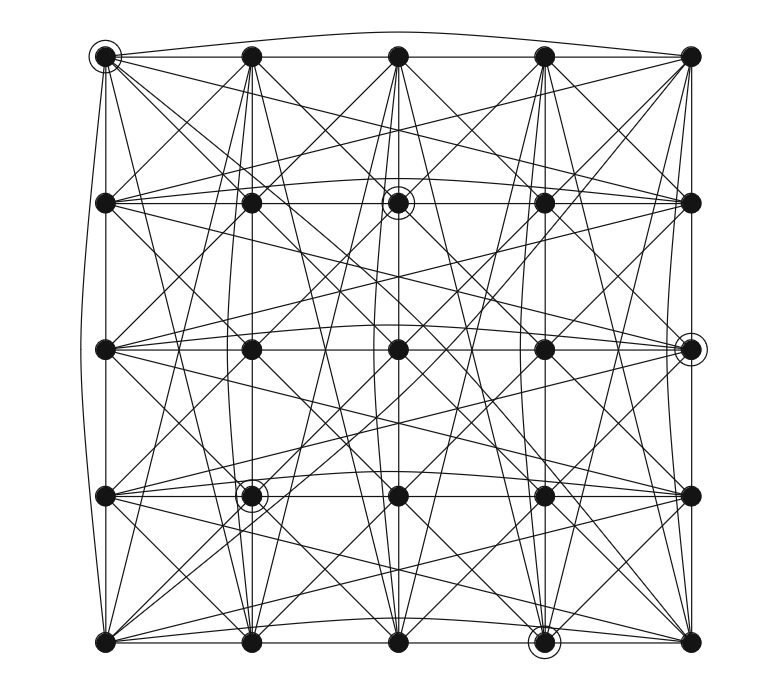
\includegraphics[width=\marginparwidth-20pt]{images/C5xC5.png}\vspace*{-10pt}\ \ \ \center The graph $C_5 \times C_5$}

and Shannon's problem was to compute $\Theta(G)$, and in particular $\Theta(C_5)$.


Let us look at $C_5$. So far we know $\alpha(C_5) = 2 \leq \Theta(C_5)$. Looking at 
the $5$-cycle as depicted earlier, or at the product $C_5 x C_5$ as drawn on the 
left, we see that the set $\{(1, 1), (2,3), (3,5), (4,2), (5,4)\}$ is independent 
in $C_5^2$. Thus we have $\alpha(C_5^2) \geq 5$. Since an independent set can contain 
only two vertices from any two consecutive rows we see that $\alpha(C_5^2) = 5$.
Hence, by using strings of length $2$ we have increased the lower bound for the capacity to $\Theta(C_5) \geq \sqrt{5}$.


So far we have no upper bounds for the capacity. To obtain such bounds 
we again follow Shannon's original ideas. First we need the dual definition 
of an independent set. We recall that a subset $C \subseteq V$ is a \textit{clique} if any
two vertices of $C$ are joined by an edge. Thus the vertices form trivial

%%%%%%%%%%%%%%%%%%%%%%%%%%%%%%%%%%%%%%%%%%%%%%%%%%
% THIRD PAGE
\setnewpagemargins

cliques of size $1$, the edges are the cliques of size $2$, the triangles are cliques 
of size $3$, and so on. Let $C$ be the set of cliques in $G$. Consider an arbitrary 
probability distribution $x = (x_v : v \in V)$ on the set of vertices, that 
is, $x_v \geq 0$ and $\sum_{v \in V} x_v = 1$. To every distribution $x$ we associate 
the ``maximal value of a clique"

\begin{equation*}
\lambda(x) = \max_{C \in \mathcal{C}} \sum_{v\in C} x_v.
\end{equation*}

and finally we set

\begin{equation*}
\lambda(G) = \min_x\lambda(x) = \min_x\max_{C \in \mathcal{C}} \sum_{v\in C} x_v.
\end{equation*}

To be precise we should use inf instead of min, but the minimum exists
because $\lambda(x)$ is continuous on the compact set of all distributions.
Consider now an independent set $U \subseteq V$ of maximal size $\alpha(G) = \alpha $.
Associated to $U$ we define the distribution $x_U  = (x_v : v \in V)$ by setting 
$x_v = \frac{1}{\alpha}$ if $v \in U$ and $x_v = 0$ otherwise. Since any clique contains at most 
one vertex from $U$,  we infer $\lambda(x_U) = \frac{1}{\alpha} $, 
and thus by the definition of $\lambda(G)$

\begin{equation*}
\lambda(G) \leq \frac{1}{\alpha(G)} \quad \text{or} \quad \alpha(G) \leq \lambda(G)^{-1}.
\end{equation*}

What Shannon observed is that $\lambda(G)^{-1}$ is, in fact, an upper bound for all 
$\sqrt[n]{\alpha(G^n)}$, and hence also for $\Theta(G)$. In order to prove this it suffices to 
show that for graphs $G$, $H$

\begin{equation}
\lambda(G \times H) = \lambda(G)\lambda(H) \label{one}
\end{equation}

holds, since this will imply $\lambda(G^n) = \lambda(G)^n$ and hence

\begin{equation*}
  \begin{align*}
  \alpha(G^n) \leq \lambda(G^n)^{-1} = \lambda(G)^{-n} \\
  \sqrt[n]{\alpha(G^n)} \leq \lambda(G)^{-1}.
  \end{align*}
\end{equation*}

% FIX BIBLIOGRAPHY
To prove (\ref{one}) we make use of the duality theorem of linear programming 
(see [I]) and get

\begin{equation}
  \lambda(G) = \min_x\max_{C \in \mathcal{C}} \sum_{v\in C} x_v = \max_y\min_{v \in V}\sum_{C \ni v}y_C, \label{two}
\end{equation}

where the right-hand side runs through all probability distributions $y = (y_C : C \in \mathcal{C})$
on $\mathcal{C}$.\\
Consider $G \times H$, and let $x$ and $x'$ be distributions which achieve the 
minima, $\lambda(x) = \lambda(G)$, $\lambda(x') = \lambda(H)$. In the vertex set of $G \times H$ we 
assign the value $z_{(u,v)} = x_ux'_v$ to the vertex $(u, v)$. Since $\sum_{(u,v)}z_{(u,v)} = \sum_u x_u \sum_v x'_v, = 1$, 
we obtain a distribution. Next we observe that the maximal cliques in 
$G \times H$ are of the form $C \times D = \{(u, v) : u \in C, v \in D \} $
where $C$ and $D$ are cliques in $G$ and $H$, respectively. Hence we obtain 

\begin{equation*}
  \begin{align}
  \lambda(G \times H) \leq \lambda(z)\quad =\quad \max_{C \times D} \sum_{(u,v) \in C \times D} z_(u,v)\\
  -\quad \max_{C \times D} \sum_{u\in C} x_u \sum_{v \in D} x'_v = \lambda(G)\lambda(H)
  \end{align}
\end{equation*}

%%%%%%%%%%%%%%%%%%%%%%%%%%%%%%%%%%%%%%%%%%%%%%%%%%
% FOURTH PAGE
\setnewpagemargins

by the definition of $\lambda(G \times H)$. In the same way the converse inequality 
$\lambda(G \times H) \geq \lambda(G)\lambda(H)$ is shown by using the dual expression for $\lambda(G)$ 
in (\ref{two}). In summary we can state: 

\begin{equation*}
  \Theta(G) \leq \lambda(G)^{-1},
\end{equation*}

for any graph G.
Let us apply our findings to the $5$-cycle and, more generally, to the $m$-cycle $C_m$.
By using the uniform distribution $(\frac{1}{m},\dotsb,\frac{1}{m})$ on the 
vertices, we obtain $\lambda(C_m) \leq \frac{2}{m} $, since any clique contains at most two 
vertices. Similarly, choosing $\frac{1}{m}$ for the edges and $0$ for the vertices, we have 
$\lambda(C_m) \geq \frac{2}{m}$ by the dual expression in (\ref{two}). We conclude that $\lambda(C_m) = \frac{2}{m}$ 
and therefore 

\begin{equation*}
  \Theta(C_m) \leq \frac{m}{2}
\end{equation*}

for all $m$. Now, if $m$ is even, then clearly $\alpha(C_m) = \frac{m}{2}$
and thus also $\Theta(C_m) = \frac{m}{2}$. For odd $m$, however, we have $\alpha(C_m) = \frac{m-1}{2}$. 
For $m = 3$, $C_3$ is a clique, and so is every product $C_3^n$, implying $a(C_3) = \Theta(C_3) = 1$. 
So, the first interesting case is the 5-cycle, where we know up to now 

\begin{equation}
  \sqrt{5} \leq \Theta(C_m) \leq \frac{5}{2} \label{three}
\end{equation}

Using his linear programming approach (and some other ideas) Shannon 
was able to compute the capacity of many graphs and, in particular, of all 
graphs with five or fewer vertices --- with the single exception of $C_5$, where 
he could not go beyond the bounds in (\ref{three}). This is where things stood for 
more than $20$ years until L\'aszl\'o Lov\'asz showed by an astonishingly simple argument
that indeed $\Theta(C_5) = \sqrt{5}$. A seemingly very difficult combinatorial 
problem was provided with an unexpected and elegant solution.\\

Lov\'asz' main new idea was to represent the vertices $v$ of the graph by 
real vectors of length $1$ such that any two vectors which belong to nonadjacent 
vertices in $G$ are orthogonal. Let us call such a set of vectors 
an orthonormal representation of $G$. Clearly, such a representation always 
exists: just take the unit vectors $(1,0,\dotsb,0)^T$, $(0,1,0,\dotsb,0)^T$, \dotsb,
$(0,0,\dotsb,1)^T$ of dimension $m=|V|$.\\


For the graph $C_5$ we may obtain an orthonormal representation in $\mathbb{R}^3$ by 
considering an ``umbrella" with five ribs $v_1, \dotsb , v_5$ of unit length. Now 
open the umbrella (with tip at the origin) to the point where the angles 
between alternate ribs are $90^\circ$. \\
Lov\'asz then went on to show that the height $h$ of the umbrella, that is, the 
distance between $0$ and $S$, provides the bound

% ADD IMAGE IN THE LEFT MARGIN
\marginnote{\hspace*{-1cm}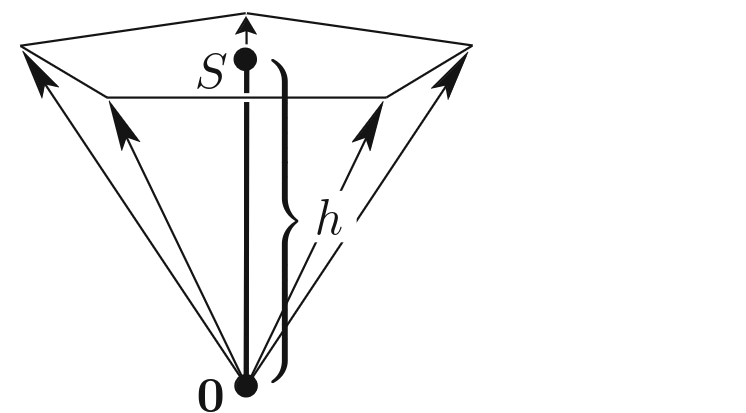
\includegraphics[width=\marginparwidth-30pt]{images/umbrella.png}\vspace*{-8pt}\\\center\hspace*{-40pt}\footnotesize{The Lov\'asz umbrella}}[-2cm]

\begin{equation}
  \Theta(C_5) \leq \frac{1}{h^2}. \label{four}
\end{equation}

A simple calculation yields $h^2 = \frac{1}{5}$; see the box on the next page. From   
this $\Theta(C_5) \leq \sqrt{5}$ follows, and therefore $\Theta(C_5) = \sqrt{5}$.

%%%%%%%%%%%%%%%%%%%%%%%%%%%%%%%%%%%%%%%%%%%%%%%%%%
% FIFTH PAGE

\setnewpagemargins

Let us see how Lov\'asz proceeded to prove the inequality (\ref{four}). (His results 
were, in fact, much more general.) Consider the usual inner product 

\begin{equation*}
  \langle x,y \rangle = x_1y_1 + \dotsb + x_8y_8
\end{equation*}

of two vectors $x = (x_1, \dotsb, x_s)$, $y = (y_1, \dotsb, y_s)$ in $\mathbb{R}^s$.
Then $|x|^2 = \langle x,x \rangle = x_1^2 + \dotsb + x_s^2$ is the square of the length $|x|$
of $x$, and the angle $\gamma$ between $x$ and $y$ is given by

\begin{equation*}
  \cos \gamma = \frac{\langle x,y \rangle}{|x||y|}.
\end{equation*}

Thus $\langle x,y \rangle = 0$ if and only if $x$ and $y$ are orthogonal.\\

% ADD IMAGES IN THE RIGHT MARGIN
\marginnote{\hspace*{8pt}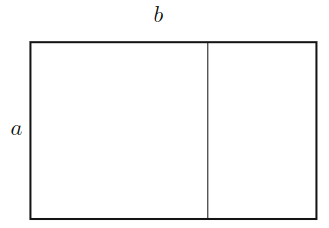
\includegraphics[width=\marginparwidth-40pt]{images/rectangle.png}\\\vspace*{-5pt}\hspace*{135pt}$b - a$}[28pt]
\marginnote{\hspace*{8pt}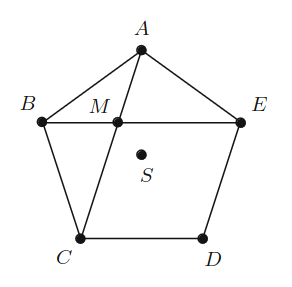
\includegraphics[width=\marginparwidth-70pt]{images/pentagon.png}\\\center\hspace*{-0.8cm}}[178pt]

\begin{mdframed}[nobreak=true]
\vspace{8pt}
{\Large\textbf{Pentagons and the golden section}}\\
[5pt]
Tradition has it that a rectangle was considered aesthetically pleasing 
if, after cutting off a square of length $a$, the remaining rectangle had 
the same shape as the original one. The side lengths $a$, $b$  of such a
rectangle must satisfy $\frac{b}{a}= \frac{a}{b-a}$. Setting $\tau := \frac{b}{a}$
for the ratio, we obtain $\tau = \frac{1}{\tau-1}$ or $\tau^2 - \tau - 1 = 0$. Solving
the quatratic equation yields the \textit{golden section} $\tau = \frac{1 + \sqrt{5}}{2}$ \approx 1.6180.\\

Consider now a regular pentagon of side length $a$, and let $d$ be the 
length of its diagonals. It was already known to Euclid (Book XIII,8) 
that $\frac{d}{a} = \tau$, and that the intersection point of two diagonals divides 
the diagonals in the golden section.\\

Here is Euclid's Book Proof. Since the total angle sum of the pentagon 
is $3\pi$, the angle at any vertex equals $\frac{3\pi}{5}$. It follows that 
$\sphericalangle ABE = \frac{\pi}{5}$, since $ABE$ is an isosceles triangle. This, in turn, 
implies $\sphericalangle AMB = \frac{3\pi}{5}$, and we conclude that the triangles $ABC$ and 
$AMB$ are similar. The quadrilateral $CMED$  is a rhombus since opposing sides are
parallel (look at the angles), and so $|MC| = a$ and thus $|AM| = d - a$. By the similarity of 
$ABC$ and $AMB$ we conclude

\begin{equation*}
  \frac{d}{a} = \frac{|AC|}{|AB|} = \frac{|AB|}{|AM|} = \frac{a}{b-a} = \frac{|MC|}{|MA|} = \tau.
\end{equation*}

There is more to come. For the distance $s$ of a vertex to the center of 
the pentagon $S$,  the reader is invited to prove the relation $s^2 = \frac{d^2}{\tau + 2}$ 
(note that $BS$ cuts the diagonal $AC$ at a right angle and halves it). 
To finish our excursion into geometry, consider now the umbrella 
with the regular pentagon on top. Since alternate ribs (of length $1$) 
form a right angle, the theorem of Pythagoras gives us $d = \sqrt{2}$, and 
hence $s^2 = \frac{2}{\tau + 2} = \frac{4}{\sqrt{5} + 5}$. So, with Pythagoras again, 
we find for the height $h = |OS|$ our promised result

\begin{equation*}
  h^2 = 1 - s^2 = \frac{1+\sqrt{5}}{\sqrt{5}+5} = \frac{1}{\sqrt{5}}.
\end{equation*}

\vspace{5pt}

\end{mdframed}

%%%%%%%%%%%%%%%%%%%%%%%%%%%%%%%%%%%%%%%%%%%%%%%%%%
% SIXTH PAGE

\setnewpagemargins

Now we head for an upper bound ``$\Theta(G) \leq \sigma^{-1}$" for the Shannon capacity
of any graph $G$ that has an especially ``nice" orthonormal representation.
For this let $T = \{v^{(1)},\ldots,v^{(m)}\}$ be an orthonormal representation 
of $G$ in $\mathbb{R}^{s}$, where $v^{(i)}$ corresponds to the vertex $v_i$. We assume in
adition that all the vectors $v^{(i)}$ have the same angle $(\neq 90^{\circ})$ with the
vector $u := {\frac{1}{m}}(v^{(1)}+\ldots+v^{(m)})$, or equivalently that the inner product 

\[
 \langle v^{(i)}, u\rangle  = \sigma _T
\]

has the same value $\sigma_T \neq 0$ for all $i$. Let us call this value $\sigma_T$ the \textit{constant}
of the representation $T$. For the Lov\'asz umbrella that represents $C_5$ the 
condition $\langle v^{(i)},u \rangle = \sigma_T$ certainly holds, for $u = \overset{\rightarrow}{OS}$.\\
Now we proceed in the following three steps.\\
$\mathbf{(A)}$ Consider a probability distribution $x = (x_1,\ldots, x_m)$ on $V$ and set

\[
\mu(x) := \quad |x_1v^{(1)}+\ldots+x_mv^{(m)}|^{2},
\]

and

\[
{\mu_{T}}(G) := \underset{x}{\inf}\mu(x).
\]

Let $U$ be a largest independent set in $G$ with $|U| = a$, and define
$x_U = (x_1,\ldots,x_m)$ with $x_i = {\frac{1}{\alpha}}$ if $v_i\in U$ and $x_i = 0$  otherwise. Since all 
vectors $v^{(i)}$  have unit length and $\langle v^{(i)}, v^{(j)} \rangle = 0$ for any two non-adjacent 
vertices, we infer

\[
    \mu_T(G)\leq\mu(x_U)=|\sum_{i=1}^{m}x_iv^{(i)}|^2= \sum_{i=1}^{m} {x_i}^2 = \alpha {\frac{1}{\alpha^{2}}} = {\frac{1}{\alpha}}.
\]

Thus we have $\mu_{T}(G) \leq \alpha^{-1}$ , and therefore

\[
    \alpha(G) \leq {\frac{1}{\mu_{T}(G)}}.
\]

$\mathbf{(B)}$ Next we compute ${\mu_T}(G)$. We need the Cauchy-Schwarz inequality

\[
\langle a,b \rangle^2 \leq |a|^2 |b|^2
\]

for vectors $a,b \in \mathbb{R}^s$. Applied to $a = x_{1}v^{(1)}+\ldots+x_{m}v^{(m)}$ and $b=u$,
the inequality yields

\begin{equation}
  \langle x_{1}v^{(1)}+\ldots+x_{m}v^{(m)},u \rangle ^2 \leq \mu(x) |u|^2. \label{five} \label{five}
\end{equation}

By our assumption that $\langle v^{(i)}, u \rangle = \sigma_T$ for all $i$, we have

\[
\langle x_{1}v^{(1)}+\ldots+x_{m}v^{(m)},u\rangle = (x_1 + \ldots + x_m)\sigma_T = \sigma_T
\]

for any distribution $x$. Thus, in particular, this has to hold for the uniform 
distribution $(\frac{1}{m}, \ldots, \frac{1}{m})$,which implies $|u|^2 = \sigma_T$.
Hence (\ref{five}) reduces to 

\begin{equation*}
\sigma_T^2 \leq \mu(x)\sigma_T \quad \text{or} \quad \mu_{T}(G) \geq \sigma_T.
\end{equation*}

%%7th page
\setnewpagemargins
On the other hand, for $x = (\frac{1}{m}, \ldots, \frac{1}{m})$  we obtain

\[
\mu_{T}(G) \leq \mu(x) = |{\frac{1}{m}}(v^{(1)}+\ldots+v^{(m)})|^2 = |u|^2 = \sigma_T,
\]

and so we have proved 

\begin{equation}
\mu_{T}(G) = \sigma_T. \label{six}
\end{equation}

In summary, we have established the inequality 

\begin{equation}
    \alpha(G) \leq {\frac{1}{\sigma_T}} \label{seven}  
\end{equation}

for any orthonormal respresentation $T$ with constant $\sigma_T$.\\
$\mathbf{(C)}$ To extend this inequality to $\Theta(G)$, we proceed as before. Consider 
again the product $G \times H$ of two graphs. Let $G$ and $H$ have orthonormal 
representations $R$ and $S$ in $\mathbb{R}^r$ and $\mathbb{R}^s$, respectively, with constants $\sigma_R$ and $\sigma_S$.
Let $v = (v_1,\ldots,v_r)$ be a vector in $R$ and $w = (w_1,\ldots,w_s)$ be 
a vector in $S$. To the vertex in $G \times H$ corresponding to the pair $(v, w)$ we 
associate the vector

\[
vw^T := ({v_1}{w_1},\ldots,{v_1}{w_s},{v_2}{w_1},\ldots,{v_2}{w_s},\ldots,{v_r}{w_1},\ldots,{v_r}{w_s}) \in \mathbb{R}^{rs}.
\]

It is immediately checked that $R \times S := \{vw^T : v \in R, w \in S\}$ is an
orthonormal representation of $G \times H$ with constant $\sigma_R \sigma_S$. Hence by (\ref{six}) 
we obtain 

\[
\mu_{R \times S}(G \times H) = \mu_{R}(G)\mu_{S}(H).
\]

For $G^n = G \times \ldots \times G$ and the representation T with constant $\sigma_T$ this
means 

\[
\mu_{T^n}(G^n) = \mu_{T}(G)^n = \sigma_{T}^n
\]

and by (\ref{seven}) we obtain

\marginnote{\hspace*{10pt}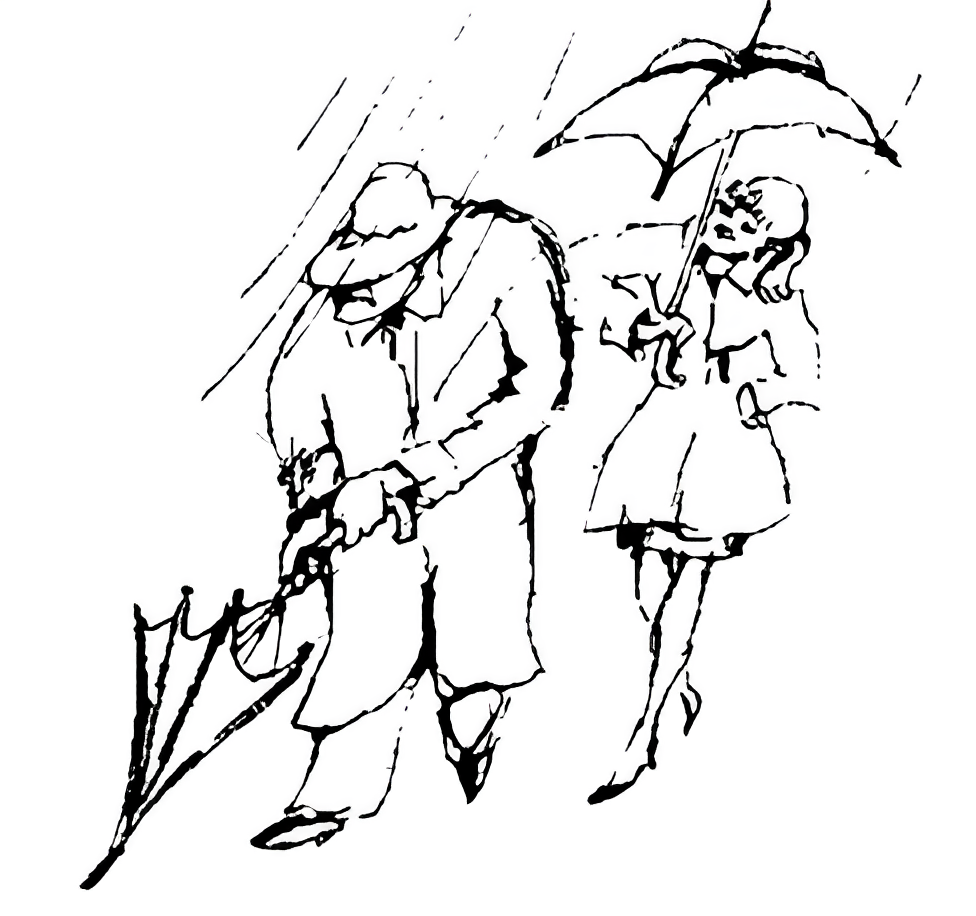
\includegraphics[width=\marginparwidth-30pt]{images/rainman.png}\\\hspace*{10pt}\textit{``Umbrellas with five ribs''}}[0pt]

\[
\alpha(G^n) \leq \sigma_{T}^{-n},  \quad   \sqrt[n]{\alpha(G^n)} \leq \sigma_{T}^{-1}.
\]

Taking all things together we have thus completed Lov\'asz' argument: 


\begin{thm}\label{theorem}
whenever $T = \{v^{(1)}, \ldots, v^{(m)}\}$) is an orthonormal\\ 
representation of $G$ with constant $\sigma_T$, then

\begin{equation}
    \Theta(G) \leq {\frac{1}{\sigma_T}}. \label{eight}
\end{equation}

\end{thm}

Looking at the Lov\'asz umbrella, we have $u = (0, 0, h = {\frac{1}{\sqrt[4]{5}}})^T$ and hence
$\sigma = \langle v^{(i)}, u \rangle = h^2 = {\frac{1}{\sqrt{5}}}$, which yields $\Theta(C_5) \leq \sqrt{5}$. Thus Shannon's 
problem is solved.


%8th page
\setnewpagemargins

\hspace{-140pt}\marginnote{
      \vspace*{0.7cm}
    \begin{equation*}
      A = 
      \begin{pmatrix}
      \ \ 0 & 1 & 0 & 0 & 1\ \ \\
      \ \ 1 & 0 & 1 & 0 & 0\ \ \\
      \ \ 0 & 1 & 0 & 1 & 0\ \ \\
      \ \ 0 & 0 & 1 & 0 & 1\ \ \\
      \ \ 1 & 0 & 0 & 1 & 0\ \ \\
      \end{pmatrix}
    \end{equation*}
    \footnotesize{The adjacency matrix for the $5$-cycle $C_5$}
}

Let us carry our discussion a little further. We see from (\ref{eight}) that the larger $\sigma_T$
is for a representation of $G$, the better a bound for $\Theta(G)$ we will get. Here 
is a method that gives us an orthonormal representation for \textit{any} graph $G$. 
To $G = (V, E)$ we associate the adjacency matrix $A = (a_{ij})$, which is 
defined as follows: Let $V = \{v_1,\ldots,v_m\}$, then we set

\[
a_{ij} := \left\{ \begin{array}{rcl}
  1 & \mbox{if $v_i v_j \in E$}\\
  0 & \mbox{otherwise.}
  \end{array}\right.
\]

$A$ is a real symmetric matrix with $0$'s in the main diagonal.\\ 
Now we need two facts from linear algebra. First, as a symmetric matrix, 
$A$ has $m$ real eigenvalues $\lambda_1 \geq \lambda_2 \geq \ldots \geq \lambda_m$ \spaceskip(some of which may be equal),
and the sum of the eigenvalues equals the sum of the diagonal 
entries of $A$, that is, 0. Hence the smallest eigenvalue must be negative 
(except in the trivial case when $G$ has no edges). {Let $p = |\lambda_m| = -\lambda_m$} be 
the absolute value of the smallest eigenvalue, and consider the matrix

\[
M := 1 + {\frac{1}{p}}A,
\]

where $I$ denotes the $(m \times m)$-identity matrix. This $M$ has the eigenvalues
$1+{\frac{\lambda_1}{p}} \geq 1+{\frac{\lambda_2}{p}} \geq \ldots \geq 1+{\frac{\lambda_m}{p}} =0$. Now we quote the second result (the principal axis theorem of linear algebra):
If $M = (m_{ij})$ is a real symmetric matrix with all eigenvalues $\geq 0$,
then there are vectors $v^{(1)}, \ldots, v^{(m)} \in \mathbb{R}^s$
for $s = \text{rank}(M)$, such that 

\[
m_{ij} = \langle v^{(i)}, v^{(j)} \rangle  \quad  (1 \leq i,j \leq m).
\]

In particular, for $M = I + {\frac{1}{p}}A$ we obtain

\[
\langle v^{(i)}, v^{(i)} \rangle = m_{ii} = 1  \quad \text{for all }i
\]

and

\[
\langle v^{(i)}, v^{(j)} \rangle = {\frac{1}{p}}a_{ij} \quad \text{for }i \neq j.
\]

Since $a_{ij} = 0 $ whenever $ v_i v_j \notin E$, we see that the 
vectors $v^{(1)},\ldots,v^{(m)}$ form indeed an orthonormal representation of $G$.\\[5pt]
Let us, finally, apply this construction to the $m$-cycles $C_m$ for odd $m > 5$. 
Here one easily computes $p = |\lambda_{min}| = 2\cos{\frac{\pi}{m}}$ (see the box). Every 
row of the adjacency matrix contains two $1$'s, implying that every row of 
the matrix $M$ sums to $1 + {\frac{2}{p}}$. For the representation $\{ v^{(1)}, \ldots, v^{(m)}\}$ this
means

\[ 
    \langle v^{(i)},v^{(1)}+ \ldots + v^{(m)} \rangle=1+{\frac{2}{p}}=1+{\frac{1}{\cos{\frac{\pi}{m}}}}
\]

and hence 
\vspace{-20pt}

\[
\langle v^{(i)},u \rangle = {\frac{1}{m}}(1+(\cos{\frac{\pi}{m}})^{-1})=\sigma
\]

for all $i$. We can therefore apply our main result (\ref{eight}) and conclude

\begin{equation}
    \Theta(C_m) \leq {\frac{m}{1+(\cos{\frac{\pi}{m}})^{-1}}} \quad\quad\quad (\text{for $m \geq 5$ odd}).\label{nine}    
\end{equation}


%9th page
\setnewpagemargins

Notice that because of $\cos{\frac{\pi}{m}} < 1$ the bound (\ref{nine}) is better than the bound 
$\Theta(C_m) \leq {\frac{m}{2}}$ we found before. Note further $\cos{\frac{\pi}{5}} = {\frac{\tau}{2}}$, where $\tau = {\frac{\sqrt{5}+1}{2}}$
is the golden section. Hence for $m = 5$ we again obtain

\[
\Theta(C_5) \leq {\frac{5}{1 + {\frac{4}{\sqrt{5}+1}}}}={\frac{5(\sqrt{5}+1)}{5+\sqrt{5}}} = \sqrt{5}.
\]

The orthonormal representation given by this construction is, of course, 
precisely the ``Lov\'asz umbrella."\\

\marginnote{%
    \hspace*{12pt}\small{For example, for $m = 7$ all we know is} \\
    \vspace{-0.2cm} % Adjust the vertical space here
    \begin{equation*}
        \hspace*{-40pt}\sqrt[5]{344} \leq \Theta(C_7) \leq \frac{7}{1+(\cos{\frac{\pi}{7}})^{-1}},
    \end{equation*}
    \hspace*{12pt}which is \ \ $3.2141 \leq \Theta(C_7) \leq 3.3177$.
}

And what about $C_7, C_9,$ and the other odd cycles? By considering $\alpha(C_m^2)$,
$\alpha(C_m^3)$ and other small powers the lower bound ${\frac{m-1}{2}} \leq \Theta(C_m)$ ) can cer-
tainly be increased, but for no odd $m \geq 7$  do the best known lower bounds
agree with the upper bound given in (\ref{eight}). So, twenty years after Lov\'asz' 
marvelous proof of $\Theta(C_5) = \sqrt{5}$, these problems remain open and are 
considered very difficult \text{---} but after all we had this situation before.\\

\begin{mdframed}[nobreak=true]
\vspace{8pt}
{\Large\textbf{The eigenvalues of $C_m$}}
\vspace{5pt}

Look at the adjacency matrix $A$ of the cycle $C_m$. To find the eigenvalues 
(and eigenvectors) we use the $m$-th roots of unity. These are 
given by $1, \zeta, \zeta^2, \ldots, \zeta^{m-1}$ for $\zeta = e^{\frac{2\pi i}{m}}$ --- see the box on page 25.\\ 
Let $\lambda \quad=\quad\zeta ^k$ \ \ be\ \  any\ \  of\ \  these roots, then we claim that
$(1, \lambda, \lambda^2, \ldots, \lambda^{m-1})^T$ is an eigenvector of $A$ to the eigenvalue $\lambda + \lambda^{-1}$.
In fact, by the set-up of $A$ we find\\

\[
A \begin{pmatrix}
    \begin{array}{@{}*{5}{l}@{}}
    1 \\
    \lambda \\
    \lambda^2 \\
    \vdots \\
    \lambda^{m-1}
    \end{array}
\end{pmatrix}
=
\begin{pmatrix}
    \begin{array}{@{}*{5}{l}@{}}
    \lambda & + & \lambda^{m-1} \\
    \lambda^2 & + & 1 \\
    \lambda^3 & + & \lambda \\
    \vdots & & \vdots \\
    1 & + & \lambda^{m-2}
    \end{array}
\end{pmatrix}
=
(\lambda + \lambda^{-1})
\begin{pmatrix}
    \begin{array}{@{}*{5}{l}@{}}
    1 \\
    \lambda \\
    \lambda^2 \\
    \vdots \\
    \lambda^{m-1}
    \end{array}
\end{pmatrix}
\]

Since the vectors $(1, \lambda, \ldots, \lambda^{m-1})$ are independent (they form a so-
called Vandermonde matrix) we conclude that for odd $m$

\begin{equation*}
\begin{aligned}
    \zeta^k + \zeta^{-k}&\quad = [(\cos(2k\pi / m)) + i\sin(2k\pi / m)]\\
&\quad\quad\ \  + [\cos(2k\pi/m) - i\sin(2k\pi / m)]\\
&\quad =  2\cos(2k\pi / m) \quad\quad\  (0 \leq k \leq \text{\tiny{$\frac{m-1}{2}$}})
\end{aligned}
\end{equation*}\\

are all the eigenvalues of $A$. Now the cosine is a decreasing function,
and So

\[
    2\cos({\frac{(m-1)\pi}{m}}) = -2\cos{\frac{\pi}{m}}
\]

is the smallest eigenvalue of $A$. 

\vspace{8pt}
\end{mdframed}


%%%%%%%%%%%%%%%%%%%%%%%%%%%%%%%%%%%%%%%%%%%%%%%%%%
% TENTH PAGE

\setnewpagemargins

% REFERENCES
\bibliography{refs.bib}

\end{document}
